\section{卷积神经网络}
卷积神经网络(CNN)是一个专门用于图像处理的神经网络。

\subsection{卷积层}

在 CNN 中,我们设计一个特定大小的区域称作“感受野”(Receptive field),
每一个神经元都只需要关心自己的感受野里面有什么东西。举例:
感受野为 $3\times3$,则一个神经元只需要输入一个 $3\times3\times3=27$ 维的向量,权重数目明显减少;

多个感受野的范围是可以重叠的,不同的神经元也可以有相同的感受野。

最经典的感受野设定:

\begin{itemize}
    \item 考虑一张图片所有的通道,而不是只考虑部分通道;
    \item 感受野的长和宽被称作 kernel size,如上方讨论的感受野的 kernel size 为 $3\times3$,一般不会设置很大的 kernel size;
    \item 同一个感受野会对应一组神经元,例如 64 个或 128 个;
    \item 对于两个相邻的感受野,将偏移量(采样间隔)称为 stride(步幅),这是一个超参数,通常不会很大,一般设置为 1 或 2 即可;
    \item 当感受野超出图像范围时,我们可以向感受野中做 padding(填补),一般补充为 0。
\end{itemize}

相同的特征可能会出现在图像的不同区域中,
但是这些相同的特征对应的是不同的神经元,但他们做的是相同的工作。我们是否需要让每一个区域都放若干个对应不同特征的神经元?

考虑共享参数,两个对应不同感受野的对应相同特征的神经元,让他们共享相同的参数,这样参数的数量将会大大减少。
由于两个神经元对应的感受野不同,他们的输入不一致,所以它们的输出也不会一样。

常见的共享参数的方法:对于同一层上的神经元,每一个感受野对应的神经元都只有一组参数,这组参数被称作 filter。

加入上述两个限制之后,我们得到的就是卷积层 Convolutional Layer。

另一种常见的解释方式是,定义若干个 $3 \times 3 \times \text{channel}$ 的 filter,将每个 filter 在输入的图片上做卷积操作,每次将 filter 移动 stride 长度,
如果超出图像范围时,我们可以选择进行 padding。

\begin{figure}[htbp]
    \centering
    \caption{卷积示意图}
    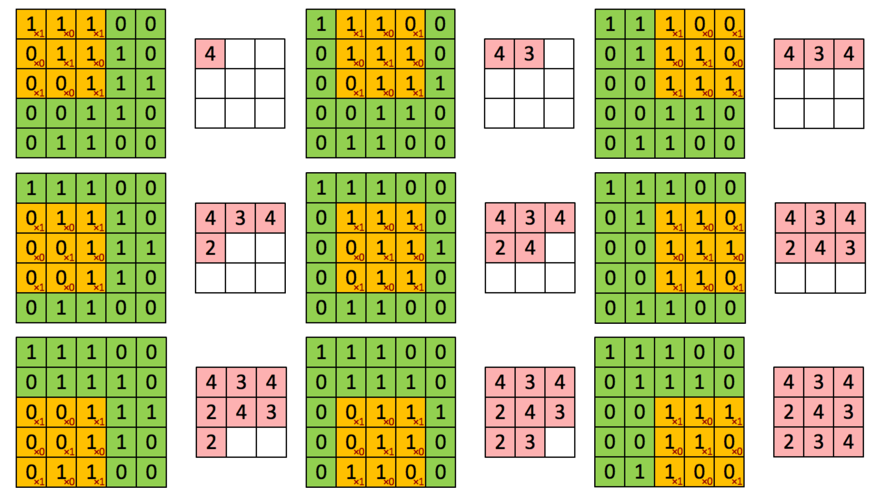
\includegraphics[scale = 0.5]{convolution.png}
\end{figure}

卷积后得到的结果被称做 Feature map。卷积之后得到的 Feature map 可以看做是一张新的图片,
只是通道数不再是输入的通道数(1 个通道 + n 个卷积核得到 n 个通道)。

当然,卷积层也是可以叠加很多层的。卷积层叠的越多,考虑的范围就会越来越大。

有时还可以在卷积之后做一次 ReLU 操作,使 Feature map 中不出现负数值结果:
\begin{equation}
    \operatorname{ReLU}(x) = \max(0, x)
\end{equation}

卷积后图像大小由下面的公式进行计算:
\begin{equation}
    \operatorname{new\_feature\_size} = \left\lfloor\operatorname{img\_size} - 
    \operatorname{filter\_size}\right\rfloor / \operatorname{stride} + 1
\end{equation}

其中,img\_size 表示原图大小,filter\_size 表示卷积核大小,stride 表示卷积核移动的步长。

\begin{example}
    输入图片规格经过预处理后尺寸为 $227 \times 227 \times 3$,
    卷积核大小为 $11 \times 11 \times 3$,步长为 $4$,则经过卷积后得到的特征图大小为
    \begin{equation*}
        \left\lfloor227 - 11\right\rfloor / 4 + 1 = 55
    \end{equation*}
    即得到的特征图的尺寸为 $55 \times 55 \times 3$。
\end{example}

\subsection{池化层}
我们观察到,有时对于一张图片,我们对其做下采样(按照一定规律在图片中采样,使图片尺寸缩小),得到的图片特征是不变的。

根据此,我们可以对卷积得到的 Feature map 通过池化层进行压缩。

我们选取一个窗口大小(通常是 $2\times2$ 或 $3\times3$),然后选择步幅(通常选择 2),
对每个窗口中的所有数取 $\max$,最终得到一个特征不变但是尺寸变小的一个 Feature map。

池化可以减少运算量,但相应的可能会损失掉一些细微的特征。池化可以改善结果,使之不容易过拟合。

经过几次卷积和池化后,我们将得到的 Feature map “拉直”(flatten)为一个向量,丢进全连接层,最后通过一个 softmax 回归器来得到最终的投票结果。

\begin{figure}[htbp]
    \centering
    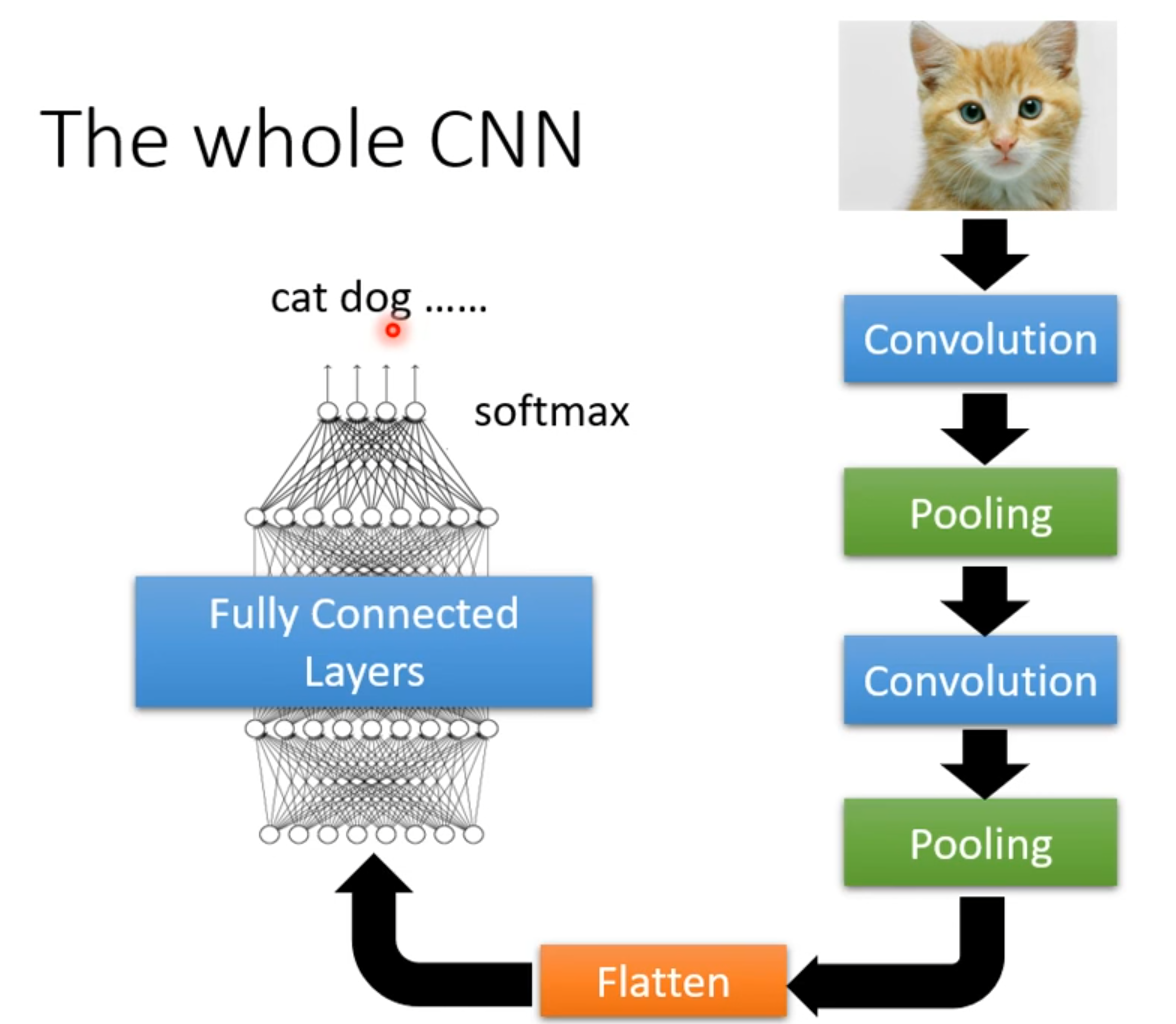
\includegraphics[scale = 0.25]{CNN.png}
\end{figure}

\subsection{超参数}
\begin{itemize}
    \item 卷积层:卷积核的数量;卷积核的大小;卷积核移动的步长
    \item 池化层:窗口的大小;窗口移动的步长
    \item 全连接层:神经元个数
\end{itemize}

\subsection{卷积神经网络的推广}
不仅是图片,卷积神经网络也可以用于其他类型的数据,比如文本、语音、视频等。
只要数据可以用矩阵表示,就可以用卷积神经网络来处理。